The NINJA-1 project was a huge success in bringing the numerical
relativity and gravitational-wave astronomy communities together.  The
project also resulted in several intriguing qualitative results.
However, it only began the process of testing detection and parameter
estimation pipelines against realistic signals.  The follow-up
project, NINJA-2, is ongoing as of the time of writing.  NINJA-2 aims
to remove many of the shortcomings of NINJA-1 and allow quantitative
studies of the behaviors of pipelines in various regions of signal
parameter space.  Specifically, NINJA-2 addresses issues with both the
waveform submissions and the noise used to construct the data sets.

\section{Hybrid pN/NR waveforms}

NINJA-1 had an open policy towards waveform submission in order to
encourage wide participation.  This meant there were no requirements
on either waveform quality or length.  The lack of quality
requirements can be seen in some of the waveforms in
figure~\ref{fig:NR-Reh22}.  There may also be less visible
implications, as there was no requirement to perform the kind of
convergence testing reported in section~\cite{sec:PNNRHybridWaveform}
although such validation is typically done by numerical relativity
groups.  The loose requirements limited the conclusions that could be
drawn, for example it makes it difficult to say whether an injection
was missed due to laying outside the region of parameter space to
which a search is sensitive, or due to an unintended feature of the
waveform.

The lack of length requirement limited the available mass range to $M
< 36 \msun$ for reasons that can be seen in
figure~\ref{fig:StildesAndInitialPSD}.   Had the waveform in that plot
not had a post-Newtonian component, the NR component to the right of
the triangles would have had to be placed below 40 Hz in order to
prevent turning on in-band.  This mass range limited the tests that
could be done, notably it entirely excluded the standard CBC
low-mass pipeline.

To address these issues NINJA-2 specifies the following minimal
requirements~\cite{ninja2-wiki}.  The raw numerical simulation should
include at least five orbits of usable data before merger (i.e., not
counting bursts of junk radiation or other significant noise).  Given
the computation cost of extending the NR waveforms, we instead require
stitching to a post-Newtonian inspiral approximant, which should be
performed at a GW frequency of $M\omega ≤ 0.075$, where $M\omega$ is
the frequency of the $(l = 2, m = \pm 2)$ harmonic. The full waveform
should be long enough to be entirely within the sensitive bands of
LIGO and Virgo down to $10 \msun$ with a lower cutoff frequency of 10
Hz, which corresponds to a starting GW frequency of $M\omega = 0.003$.
The numerical-waveform (before any hybridization) amplitude should be
accurate to within 5\%, and the phase (as a function of GW frequency)
should have an accumulated uncertainty over the entire inspiral,
merger and ringdown, of no more than 0.5 radian. The PN approximants
used for hybridization should ideally use the highest PN orders
available, both in phase and amplitude.  

These minimal accuracy requirements are motivated by the results of
the Samurai project~\cite{Hannam:2009hh}, and studies performed in
preparation for the NR-AR collaboration project~\cite{ninja-wiki}.
The question of how many NR cycles are needed in order to produce a
robust waveform is an area of current research~\ref{MacDonald:2011}. 

The NINJA-2 project encourages the inclusion of higher-order modes
above $(2,2)$, although this is not required.  We chose to restrict
attention to non-spinning waveforms and waveforms with spins aligned
or anti-aligned with the orbital angular momentum.  There are
sufficient open questions regarding these restricted cases to make
this analysis interesting, without adding the additional complications
on both the waveform generation and data analysis sides associated
with precession. 

A total of 60 waveforms from 8 groups were contributed, these are
summarized in tables ~\ref{tab:ninja2_bam}, \ref{tab:ninja2_fau},
\ref{tab:ninja2_gatech}, \ref{tab:ninja2_lean},
\ref{tab:ninja2_llama}, \ref{tab:ninja2_rit}, \ref{tab:ninja2_spec},
\ref{tab:ninja2_uiuc}, and a map of the parameter values is shown in
figure~\ref{f:ninja2_param_map}.

\begin{table}
\begin{center}
\begin{tabular}{|l|r|r|r|l|c|}
\hline
Run & $q$ & Spin1${}_z$ & Spin2${}_z$ & pN Approx. & Refs \\
\hline
BAM\_D10spp85\_80.T4.hyb.n2 & 1 & 0.85 & 0.85 & TaylorT4 & \cite{Hannam:2007wf,Brugmann:2008zz} \\
BAM\_D10spp85\_80.T1.hyb.n2 & 1 & 0.85 & 0.85 & TaylorT1 & \cite{Hannam:2007wf,Brugmann:2008zz} \\
BAM\_D125smm50Nep\_80.T1.hyb.n2 & 1 & -0.50 & -0.50 & TaylorT1 & \cite{Hannam:2007wf,Brugmann:2008zz} \\
BAM\_D125smm50Nep\_80.T4.hyb.n2 & 1 & -0.50 & -0.50 & TaylorT4 & \cite{Hannam:2007wf,Brugmann:2008zz} \\
BAM\_D13smm75Nep\_96.T4.hyb.n2 & 1 & -0.75 & -0.75 & TaylorT4 & \cite{Hannam:2007wf,Brugmann:2008zz} \\
BAM\_D13smm75Nep\_96.T1.hyb.n2 & 1 & -0.75 & -0.75 & TaylorT1 & \cite{Hannam:2007wf,Brugmann:2008zz} \\
BAM\_D13smm85Nep\_88.T4.hyb.n2 & 1 & -0.85 & -0.85 & TaylorT4 & \cite{Hannam:2007wf,Brugmann:2008zz} \\
BAM\_D13smm85Nep\_88.T1.hyb.n2 & 1 & -0.85 & -0.85 & TaylorT1 & \cite{Hannam:2007wf,Brugmann:2008zz} \\
BAM\_D11spp50\_96.T4.hyb.n2 & 1 & 0.50 & 0.50 & TaylorT4 & \cite{Hannam:2007wf,Brugmann:2008zz} \\
BAM\_D11spp50\_96.T1.hyb.n2 & 1 & 0.50 & 0.50 & TaylorT1 & \cite{Hannam:2007wf,Brugmann:2008zz} \\
BAM\_D10spp75\_80.T1.hyb.n2 & 1 & 0.75 & 0.75 & TaylorT1 & \cite{Hannam:2007wf,Brugmann:2008zz} \\
BAM\_D10spp75\_80.T4.hyb.n2 & 1 & 0.75 & 0.75 & TaylorT4 & \cite{Hannam:2007wf,Brugmann:2008zz} \\
BAM\_D12smm25Nep\_80.T4.hyb.n2 & 1 & -0.25 & -0.25 & TaylorT4 & \cite{Hannam:2007wf,Brugmann:2008zz} \\
BAM\_D12smm25Nep\_80.T1.hyb.n2 & 1 & -0.25 & -0.25 & TaylorT1 & \cite{Hannam:2007wf,Brugmann:2008zz} \\
BAM\_EP\_um4\_D10-n96.T4.hyb.n2 & 4 & 0.00 & 0.00 & TaylorT4 & \cite{Hannam:2007wf,Brugmann:2008zz} \\
BAM\_EP\_um4\_D10-n96.T1.hyb.n2 & 4 & 0.00 & 0.00 & TaylorT1 & \cite{Hannam:2007wf,Brugmann:2008zz} \\
BAM\_um3\_88.T4.hyb.n2 & 3 & 0.00 & 0.00 & TaylorT4 & \cite{Hannam:2007wf,Brugmann:2008zz} \\
BAM\_um3\_88.T1.hyb.n2 & 3 & 0.00 & 0.00 & TaylorT1 & \cite{Hannam:2007wf,Brugmann:2008zz} \\
BAM\_um2\_88.T1.hyb.n2 & 2 & 0.00 & 0.00 & TaylorT1 & \cite{Hannam:2007wf,Brugmann:2008zz} \\
BAM\_um2\_88.T4.hyb.n2 & 2 & 0.00 & 0.00 & TaylorT4 & \cite{Hannam:2007wf,Brugmann:2008zz} \\
BAM\_R6\_PN\_80.T1.hyb.n2 & 1 & 0.00 & 0.00 & TaylorT1 & \cite{Hannam:2007wf,Brugmann:2008zz} \\
BAM\_R6\_PN\_80.T4.hyb.n2 & 1 & 0.00 & 0.00 & TaylorT4 & \cite{Hannam:2007wf,Brugmann:2008zz} \\
BAM\_D12spp25\_96.T4.hyb.n2 & 1 & 0.25 & 0.25 & TaylorT4 & \cite{Hannam:2007wf,Brugmann:2008zz} \\
BAM\_D12spp25\_96.T1.hyb.n2 & 1 & 0.25 & 0.25 & TaylorT1 & \cite{Hannam:2007wf,Brugmann:2008zz} \\
BAM\_q2a0a025\_T\_96\_344.T1.hyb.n2.bbh & 2 & 0.25 & 0.00 & {} & \cite{,Brugmann:2008zz} \\
BAM\_q2a0a025\_T\_96\_344.T4.hyb.n2.bbh & 2 & 0.25 & 0.00 & {} & \cite{,Brugmann:2008zz} \\
\hline
\end{tabular}
\end{center}
\caption[BAM submissions to NINJA-2]{
\label{tab:ninja2_bam}
BAM submissions to NINJA-2}
\end{table}

\begin{table}
\begin{center}
\begin{tabular}{|l|r|r|r|l|c|}
\hline
Run & $q$ & Spin1${}_z$ & Spin2${}_z$ & pN Approx. & Refs \\
\hline
BAM\_hybrid\_om0.025etmq3S0.4- & 3 & 0.40 & 0.60 & TaylorT4 & \cite{none,???} \\
0\_0\_S0.6\_0\_0\_72 &  &  &  &  &  \\
\hline
\end{tabular}
\end{center}
\caption[FAU submissions to NINJA-2]{
\label{tab:ninja2_fau}
FAU submissions to NINJA-2}
\end{table}

\begin{table}
\begin{center}
\begin{tabular}{|l|r|r|r|l|c|}
\hline
Run & $q$ & Spin1${}_z$ & Spin2${}_z$ & pN Approx. & Refs \\
\hline
MayaKranc\_D12\_a0.00\_m129\_nj & 1 & 0.00 & 0.00 & TaylorT4 & \cite{,} \\
MayaKranc\_D10\_a0.90\_m129\_nj & 1 & 0.90 & 0.90 & TaylorT4 & \cite{,} \\
MayaKranc\_D10\_a0.20\_m77\_nj & 1 & 0.20 & 0.20 & TaylorT4 & \cite{,} \\
MayaKranc\_D10\_a0.60\_m77\_nj & 1 & 0.60 & 0.60 & TaylorT4 & \cite{,} \\
MayaKranc\_D12\_a0.60\_m103\_nj & 1 & 0.60 & 0.60 & TaylorT4 & \cite{,} \\
MayaKranc\_Sp02py0935th90\_gr & 1 & 0.80 & 0.00 & TaylorT4 & \cite{,} \\
MayaKranc\_D12\_a0.80\_m103\_nj & 1 & 0.80 & 0.80 & TaylorT4 & \cite{,} \\
MayaKranc\_D12\_a0.00\_q2\_m90\_nj & 2 & 0.00 & 0.00 & TaylorT4 & \cite{,} \\
MayaKranc\_D11\_a0.20\_q2\_m90\_nj & 2 & 0.02 & 0.09 & TaylorT4 & \cite{,} \\
MayaKranc\_D10\_a0.40\_m90\_nj & 1 & 0.40 & 0.40 & TaylorT4 & \cite{,} \\
MayaKranc\_D10\_a0.80\_m90\_nj & 1 & 0.80 & 0.80 & TaylorT4 & \cite{,} \\
MayaKranc\_D12\_a0.40\_m103\_nj & 1 & 0.40 & 0.40 & TaylorT4 & \cite{,} \\
MayaKranc\_D12\_a0.20\_m103\_nj & 1 & 0.20 & 0.20 & TaylorT4 & \cite{,} \\
\hline
\end{tabular}
\end{center}
\caption[GATech submissions to NINJA-2]{
\label{tab:ninja2_gatech}
GATech submissions to NINJA-2}
\end{table}

\begin{table}
\begin{center}
\begin{tabular}{|l|r|r|r|l|c|}
\hline
Run & $q$ & Spin1${}_z$ & Spin2${}_z$ & pN Approx. & Refs \\
\hline
dq4 & 4 & 0.00 & 0.00 & TaylorT1 & \cite{,Sperhake:2006cy} \\
\hline
\end{tabular}
\end{center}
\caption[LEAN submissions to NINJA-2]{
\label{tab:ninja2_lean}
LEAN submissions to NINJA-2}
\end{table}

\begin{table}
\begin{center}
\begin{tabular}{|l|r|r|r|l|c|}
\hline
Run & $q$ & Spin1${}_z$ & Spin2${}_z$ & pN Approx. & Refs \\
\hline
Llama\_d550-h64-Hybrid & 1 & 0.00 & 0.00 & 3.5pNTaylorF2 & \cite{Reisswig:2009rx,Reisswig:2009rx} \\
Llama\_d4d4-q1--D10-h64-r250.T4.hybrid & 1 & -0.40 & -0.40 & TaylorT4 & \cite{Pollney:2010hs,Pollney:2009yz,} \\
Llama\_d4d4-q1--D10-h64-r250.T1.hybrid & 1 & -0.40 & -0.40 & TaylorT1 & \cite{Pollney:2010hs,Pollney:2009yz,} \\
Llama\_u4u4-q1--D8-h64-r250.T1.hybrid & 1 & 0.40 & 0.40 & TaylorT1 & \cite{Pollney:2010hs,Pollney:2009yz,} \\
Llama\_u4u4-q1--D8-h64-r250.T4.hybrid & 1 & 0.40 & 0.40 & TaylorT4 & \cite{Pollney:2010hs,Pollney:2009yz,} \\
Llama\_d5q2-h016-Hybrid & 2 & 0.00 & 0.00 & 3.5pNTaylorF2 & \cite{,Reisswig:2009rx} \\
Llama\_u2u2-q1--D8-h64-r250.T1.hybrid & 1 & 0.20 & 0.20 & TaylorT1 & \cite{Pollney:2010hs,Pollney:2009yz,} \\
Llama\_u2u2-q1--D8-h64-r250.T4.hybrid & 1 & 0.20 & 0.20 & TaylorT4 & \cite{Pollney:2010hs,Pollney:2009yz,} \\
Llama\_d2d2-q1--D10-h64-r250.T1.hybrid & 1 & -0.20 & -0.20 & TaylorT1 & \cite{Pollney:2010hs,Pollney:2009yz,} \\
Llama\_d2d2-q1--D10-h64-r250.T4.hybrid & 1 & -0.20 & -0.20 & TaylorT4 & \cite{Pollney:2010hs,Pollney:2009yz,} \\
\hline
\end{tabular}
\end{center}
\caption[Llama submissions to NINJA-2]{
\label{tab:ninja2_llama}
Llama submissions to NINJA-2}
\end{table}

\begin{table}
\begin{center}
\begin{tabular}{|l|r|r|r|l|c|}
\hline
Run & $q$ & Spin1${}_z$ & Spin2${}_z$ & pN Approx. & Refs \\
\hline
LazEV\_D8.4\_10to1\_nj\_hybrid & 10 & 0.00 & 0.00 & TaylorT4 & \cite{Campanelli:2005dd} \\
\hline
\end{tabular}
\end{center}
\caption[RIT submissions to NINJA-2]{
\label{tab:ninja2_rit}
RIT submissions to NINJA-2}
\end{table}

\begin{table}
\begin{center}
\begin{tabular}{|l|r|r|r|l|c|}
\hline
Run & $q$ & Spin1${}_z$ & Spin2${}_z$ & pN Approx. & Refs \\
\hline
SpEC\_q6s0 & 6 & 0.00 & 0.00 & TaylorT1 & \cite{SpECWebsite} \\
SpEC\_q4s0 & 4 & 0.00 & 0.00 & TaylorT2 & \cite{SpECWebsite} \\
SpEC\_EqualMassAntiAlignedSpins & 1 & -0.44 & -0.44 & NA & \cite{chu-2009,SpECWebsite} \\
SpEC\_q1s-0.95 & 1 & -0.95 & -0.95 & TaylorT1 & \cite{SpECWebsite} \\
SpEC\_q2s0 & 2 & 0.00 & 0.00 & TaylorT2 & \cite{SpECWebsite} \\
SpEC\_EqualMassAlignedSpins & 1 & 0.44 & 0.44 & NA & \cite{chu-2009,SpECWebsite} \\
SpEC\_q3s0 & 3 & 0.00 & 0.00 & TaylorT2 & \cite{SpECWebsite} \\
SpEC\_EqualMassNonspinning & 1 & 0.00 & 0.00 & TaylorT4 & \cite{Scheel:2008rj,SpECWebsite} \\
\hline
\end{tabular}
\end{center}
\caption[SpEC submissions to NINJA-2]{
\label{tab:ninja2_spec}
SpEC submissions to NINJA-2}
\end{table}

\begin{table}
\begin{center}
\begin{tabular}{|l|r|r|r|l|c|}
\hline
Run & $q$ & Spin1${}_z$ & Spin2${}_z$ & pN Approx. & Refs \\
\hline
UIUC\_spin\_-0.25\_om0.0528\_22-HYBRID & 1 & -0.25 & -0.25 & NA & \cite{none} \\
UIUC\_spin\_0.85\_om0.0536\_22-HYBRID & 1 & 0.85 & 0.85 & NA & \cite{none} \\
\hline
\end{tabular}
\end{center}
\caption[UIUC submissions to NINJA-2]{
\label{tab:ninja2_uiuc}
UIUC submissions to NINJA-2}
\end{table}


\begin{figure}
  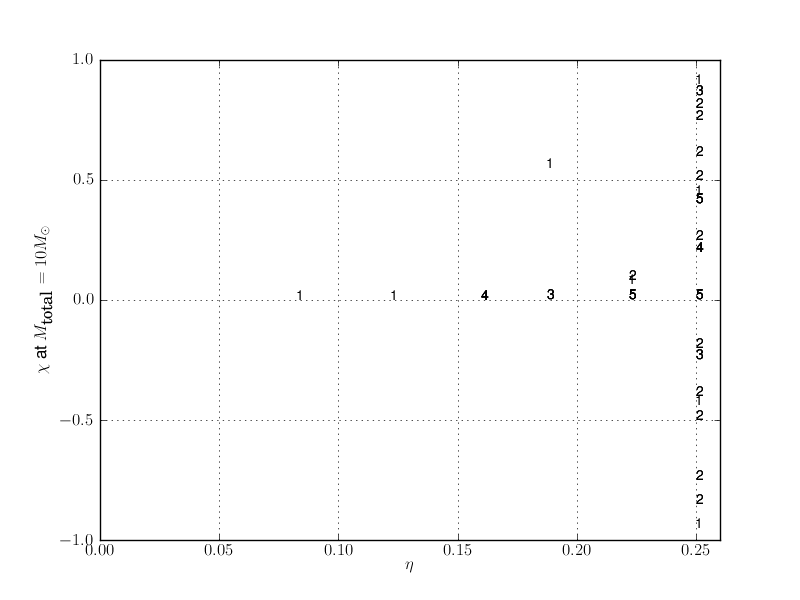
\includegraphics[width=\linewidth]{figures/ninja2/ninja2_cat.png}
  \caption[Parameters of the NINJA-2 submissions]{
  \label{f:ninja2_param_map}
Parameters of the NINJA-2 hybrid waveform submissions showing the
symmetric mass ratio $\eta=m_1 m_2 /(m_1+m_2)^2$ and dimensionless
spin parameter $\chi=(S_1/m_1 + S_2/m_2)/(m_1+m_2)$ after scaling the
waveforms to a total mass of 10 $\msun$.  The numbers indicate how
many distinct waveforms with the specified parameters were submitted.}
\end{figure}%

\subsection{Verifying the hybrid waveforms}

Each NR group verified that their waveforms met the minimum NINJA-2
requirements before submission.  Once submitted, a series of
additional checks were performed and reviewed by the entire
collaboration.  

In the first stage the post-Newtonian expressions and codes were
compared against each other and the literature.  This required several
iterations, but eventually resulted in a set of codes in various
languages that produce waveforms that all agree in both phase and
amplitude. 

In the second stage the complete hybrid waveforms were examined in the
time and frequency domains.  In the time domain we plotted the final
40 cycles of each waveform -- enough to include the full NR portion,
the hybridization region, and some of the pN portion -- and looked for
any anomalies such as those present in some of the NINJA-1 waveforms
in figure~\ref{fig:NR-Reh22}.  A few such features were indeed
visible, spotting them in this way allowed them to be corrected.  One
example, the Llama dq4 waveform is shown in
figure~\ref{f:ninja2_time_hybrids}.  In the initial version there is
an unphysical rise in the amplitude after the ringdown.  This resulted
at the stage where $h$ is obtained from $\Psi_4$ (see
sec~\ref{sec:psi4}) and was due to problems with the constants of
integration.  Once these had been set properly the unphysical feature
was removed.

\begin{figure}
  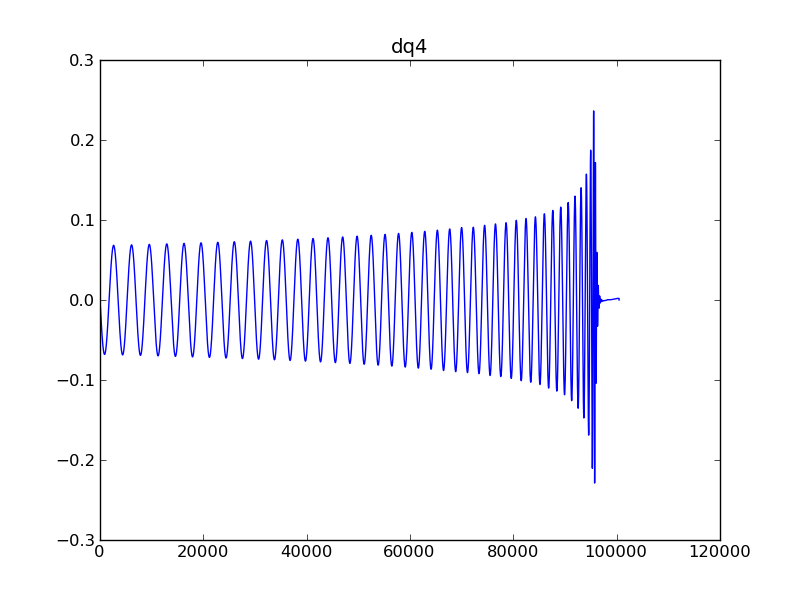
\includegraphics[width=0.5\linewidth]{figures/ninja2/dq4_before}
  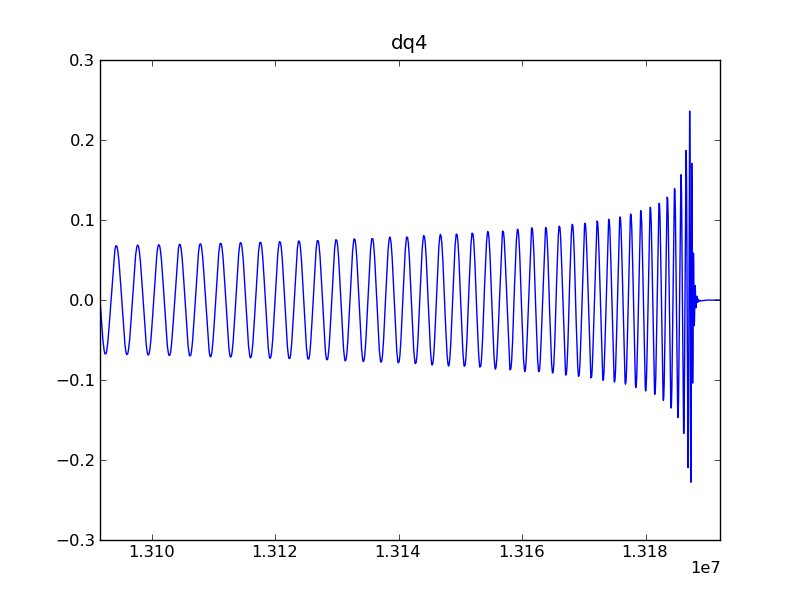
\includegraphics[width=0.5\linewidth]{figures/ninja2/dq4_after}
  \caption[Time-domain hybrid NINJA-2 waveforms]{
  \label{f:ninja2_time_hybrids}
The final 40 cycles of the $(2,2)$ mode of $h+(t)$ for the Llama
DQ4 waveform \Note{parameters}.  In the intially submitted version (left)
the amplitude does not go to zero after the ringdown.  This feature is
removed after reintegrating $\Psi_4$. \Note{Remake plots scaled to $10
\msun$}}
\end{figure}%


The amplitude of the Fourier transform of the complete waveforms were
also plotted.  This analysis also revealed unphysical features, 
primarily due to hybridization.  An example is shown in
figure~\ref{f:ninja2_freq_hybrids}, which shows a visible ``kink'' in
the waveform at the hybridization frequency, which vanishes after the
waveform was reconstructed.

\begin{figure}
  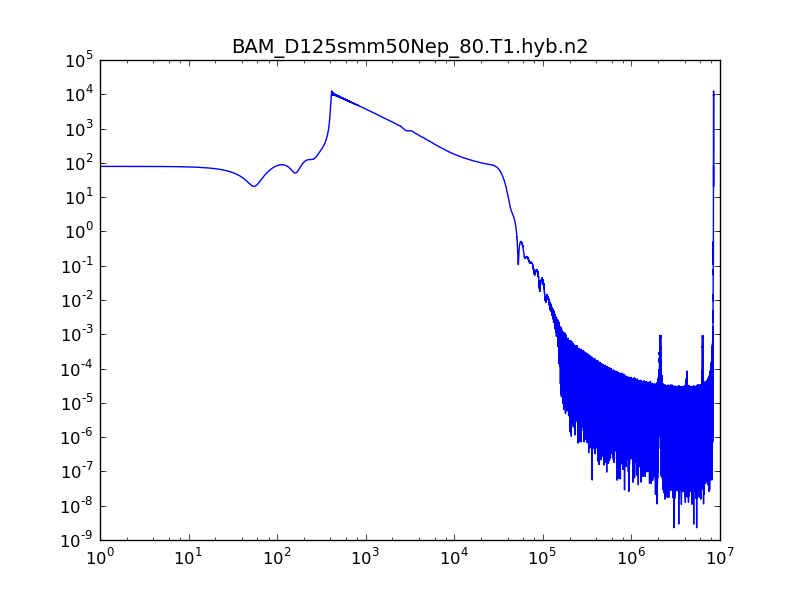
\includegraphics[width=0.5\linewidth]{figures/ninja2/bam_d125smm50nep_80_t1_hyb_n2_amp.png}
  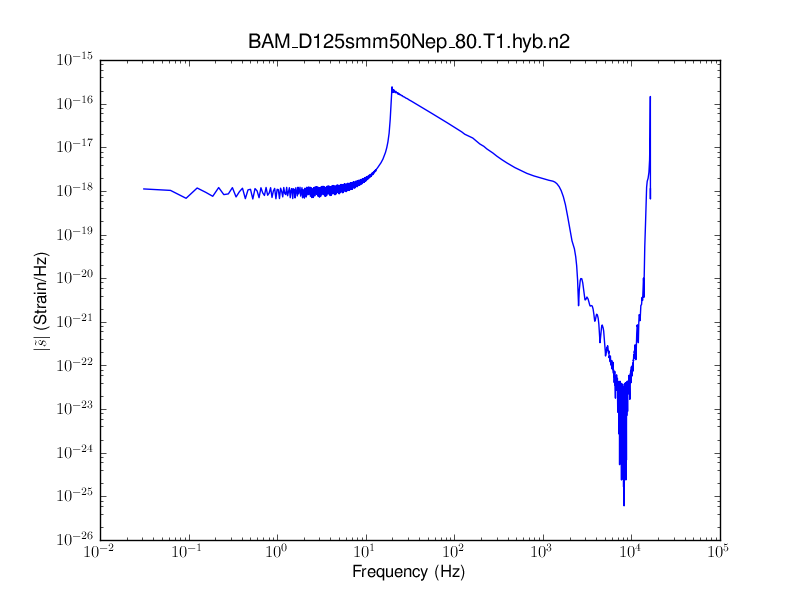
\includegraphics[width=0.5\linewidth]{figures/ninja2/bam_d125smm50nep_80_t1_hyb_n2_amp_v2.png}
  \caption[Frequency-domain hybrid NINJA-2 waveforms]{
  \label{f:ninja2_freq_hybrids}
Fourier amplitude of the $(2,2)$ mode of $h+$ for a sample NINJA-2
hybrid waveform from the BAM/AEI group \Note{parameters}.  The
waveform has been scaled to 10 $\msun$ and placed 1 Mpc from the
detector to give it physical units.  \Note{I need to dig up the old
version of the waveform and remake it with the new code} The waveform
on the left is the version initially submitted, note there is a
visible ``kink'' in the waveform at the hybridization frequency.  The
waveform on the right has been re-hybridized and there is no longer a
visible kink.  This feature did not show up in the time domain view of
the waveform.}
\end{figure}%

Finally, the waveforms were compared against each other using standard
data-analysis techniques, in particular the overlap defined in
section~\ref{sec:search_matchfilter}, using the initial LIGO noise
curve.  The waveforms were grouped into sets with identical
parameters.  For each set one waveform was chosen as the reference and
the overlap with all the other waveforms calculated over a range of
masses, optimizing over the unknown coalescence time and phase as
usual.  This process was then repeated, taking each of the other
waveforms as the reference in turn.

The initial set of contributions showed unexpectedly large mismatches
at masses $\approx 20 \msun$, at the point where the hybridization
frequency for several waveforms passes through the most sensitive
portion of the LIGO band.  This prompted a number of the NR groups to
revise their hybridization procedures, after which the overlaps were
more in line with the expected values.  A sample of these plots before
and after rehybridization is shown in
figure~\cite{f:ninja2_overlap_test}.  It is worth noting that even
after rehybridizing there are still mismatches.  In particular, the
SpEC and MayaKranc submissions use the same hybridization method, the
same pN approximant, and are simulating the same physical system.  The
overlaps approach 1 at higher masses, where the NR portion dominates.
This is an important validation, as the two groups use completely
different codes based on different principles.  The overlap is also
close to 1 at the lowest masses, where pN dominates.  This is expected
following the pN cross-checks done previously.  That the overlap
diminishes slightly at intermediate masses must be due to the
different hybridization frequencies \Note{get these values}, and
indicates the sensitivity of the waveform to the hybridization
details.


\begin{figure}
  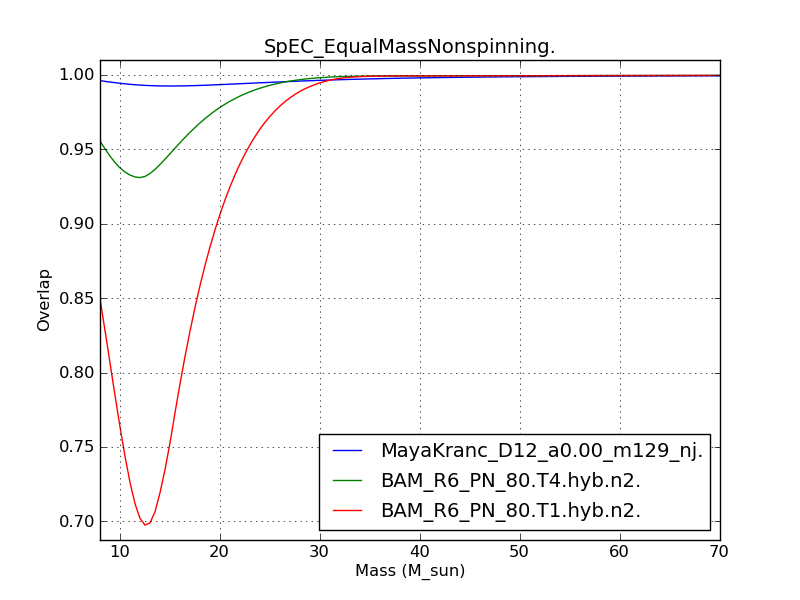
\includegraphics[width=0.5\linewidth]{figures/ninja2/q_1_z_0_figure03}
  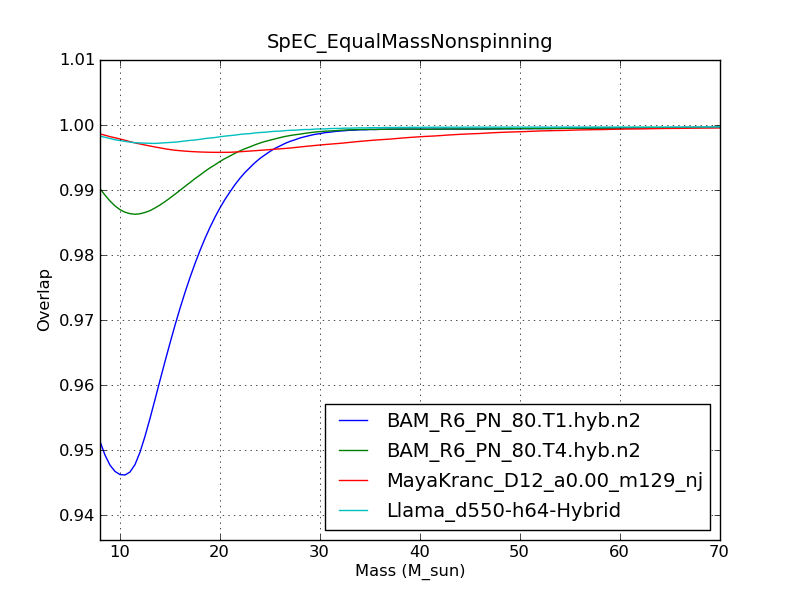
\includegraphics[width=0.5\linewidth]{figures/ninja2/figure2_1_0_16}
  \caption[Overlaps between NINJA-2 submissions maximized over time
and phase]{
  \label{f:ninja2_overlap_test}
Overlaps between the equal-mass, non-spinning NINJA-2 contributions,
maximized over time and phase.   For the original submissions (left)
overlaps are as low as 0.70 between waveforms using different pN
approximants and 0.94 for waveforms using the same approximant.  After
rehybridization (right) the waveforms achieve much higher overlaps,
with minima above 0.94 for different approximants and above 0.98 for
identical approximants.  The residual differences  between waveforms
using TaylorT4 are due to hybridization details.  The Llama waveform
was accidentally omitted from the original runs.}
\end{figure}%

We also calculated the overlaps between waveforms with identical
parameters, optimizing over mass as well as time and phase.  This gives
a sense of the range over which parameter estimation pipelines could 
be biased by unphysical features of the waveform.  Example plots
using the equal-mass, non-spinning MayaKranc waveform as the signal and
BAM plus two different approximants as the template are shown in 
figure~\ref{f:ninja2_max_over_mass_bam}.


\begin{figure}
  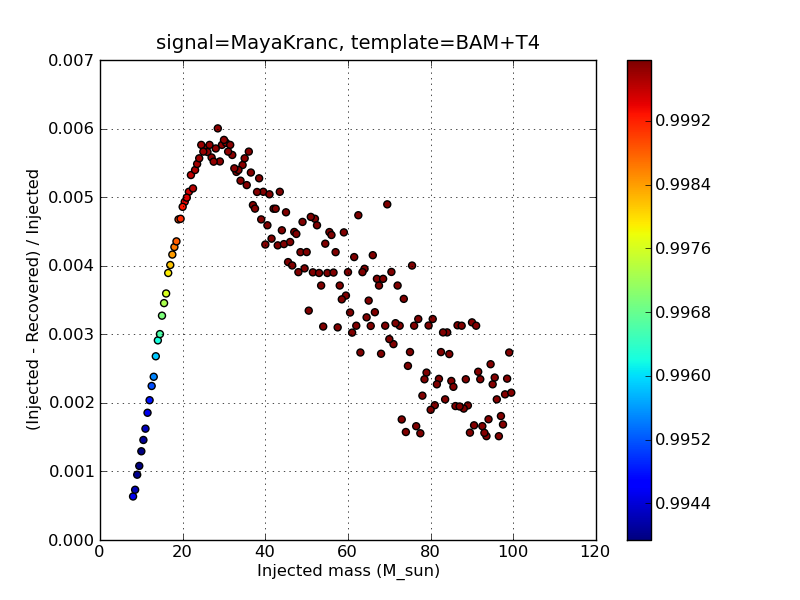
\includegraphics[width=0.5\linewidth]{figures/ninja2/maya_bamt4_max_over_m}
  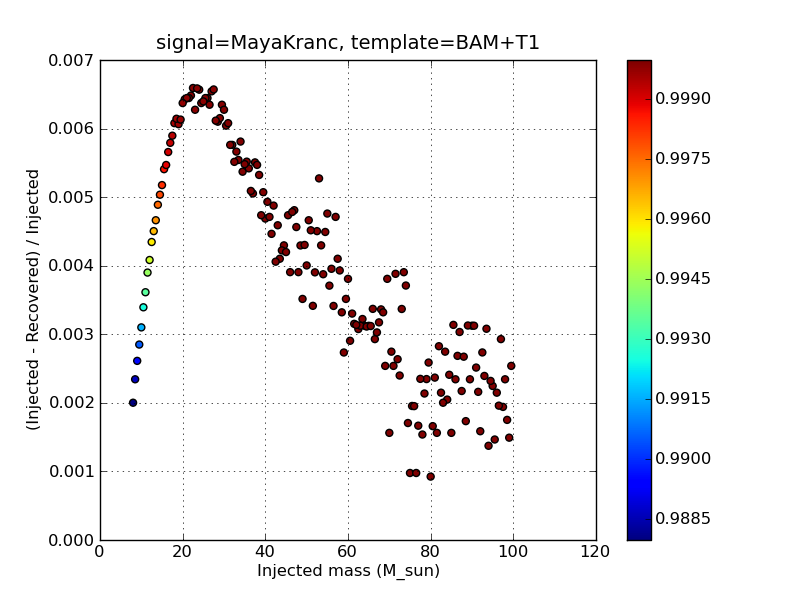
\includegraphics[width=0.5\linewidth]{figures/ninja2/maya_bamt1_max_over_m}
  \caption[Overlaps between NINJA-2 submissions maximized over mass]{
  \label{f:ninja2_max_over_mass_bam}
Overlaps between the equal-mass, non-spinning MayaKranc waveform taken
as the signal, and the equal-mass, non-spinning BAM waveform
hybridized with TaylorT4 (left) and TaylorT1 (right) taken as
templates.  Maximization is done over the mass of the template, as well
as over time and phase.  Note the lower overall overlaps and mass bias
at the low-mass end of the figure on the right, where the two different
pN waveforms dominate the overlap.}
\end{figure}%

At the high-mass end the overlap is dominated by NR data, and as in
figure~\cite{f:ninja2_overlap_test} the overlaps are high without
needing to move off the signal mass.  At the low-mass end the same
result would be expected in a pure pN/pN comparison.  However, there
is enough of the hybridization in-band to reduce the overlaps.  However,
changing the mass introduces a phase difference that accumulates over
all the cycles in-band, and so higher overlaps can not be achieved.
The result is optimal mass values close to the correct mass value, but
with a low overlap.

In the middle region these factors compete.  At higher masses the
overlap is reduced less by changing the mass and so the recovered
value can stray further from the injected value.  However as the
hybridization passes out of band this adjustment is no longer needed.


\section{Construction of the NINJA-2 data set}

In broad terms the plans for the NINJA-2 data sets follow those for
NINJA-1 (ch.~\ref{ch:ninja1}).  Simulated Gaussian noise was generated
to model the initial LIGO and Virgo noise curves, the spectra are
identical to those in figure~\ref{f:ninjapsd}.  Injection parameters,
including choice of waveform, were then selected randomly.  The
injections were then added to the Gaussian noise and distributed to
data analysis groups.  However, several key changes were made in the
details of this process in order to correct shortcomings in NINJA-1.  

The NINJA-2 data was sampled at 16384 Hz rather than the 4096 Hz used
by NINJA-1.  This was done because investigations showed that there is
power above 4096 Hz in the waveforms, which would get aliased down to 
lower frequencies if the sample rate is too low.  This problem is
illustrated in figure~\ref{f:ninja2_aliasing}.

\begin{figure}
  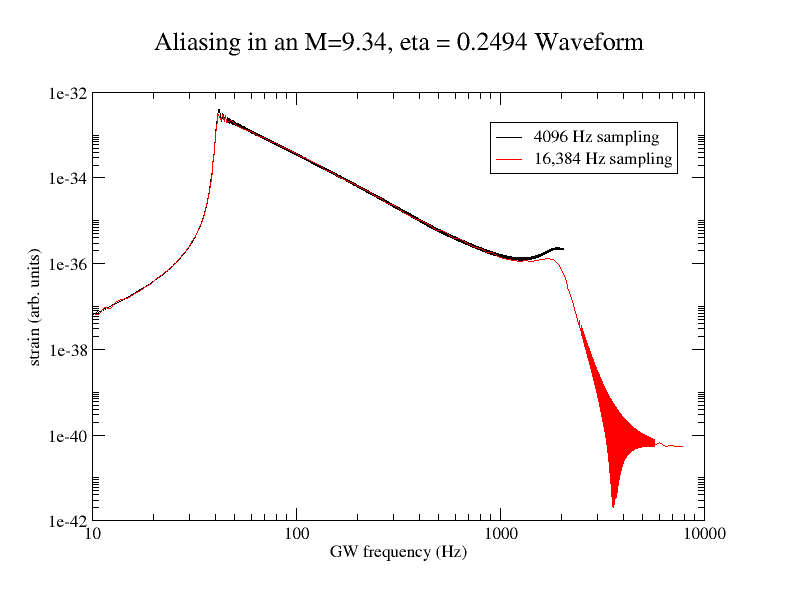
\includegraphics[width=\linewidth]{figures/ninja2/ninja2_aliasing}
  \caption[Aliasing of waveform power]{
  \label{f:ninja2_aliasing}
Frequency-domain amplitudes of a NINJA-2 waveform at different
sampling rates.  At a sample rate of 4096 Hz the late portion of the
waveform are distorted due to aliasing of power to lower frequencies.
}%

NINJA-1 consisted of only 127 injections in a day of data, which
severely limited the ability to draw statistical conclusions on the
behavior of the pipelines.  To correct this in NINJA-2 we extended the
duration to eight weeks.  The density of injections was varied over
this span:  weeks 1-3 had one injection on average every 2000 seconds,
week 4-6 had one injection on average every 4 hours, and the final two
weeks had one injection every on average every 2.5 days.  The intent
was that data analysts can tune and test their pipelines on the dense
weeks, and then optionally perform a self-blinded test on the final two
weeks.

In NINJA-1 the SNR was not chosen a priori but was determined by the
other parameters.  For NINJA-2 we draw the network SNR ($\sqrt{\sum_i
\rho_i^2}$ where $i$ ranges over the IFOs) from a distribution and
then scale the distance of the injection in order to achieve that SNR.
For the first three weeks the distribution is linear from 6 to 130 in
order to allow pipelines to test and tune out to large SNRs on the
densest set of injections.  For the remaining weeks the distribution
falls as the reciprocal of the network SNR (uniform in
$\log(\mathrm{SNR})$) in order to better model the expected
astrophysical distribution.

The mass and waveform selection were also done slightly differently in
NINJA-2.  For each injection a mass was first selected uniformly over
the specified range; for the full 2-month run this range is from
$10-350 \msun$.  Then waveforms were selected at random until one was
found that could be injected at the chosen mass such that the waveform
turns on below 35 Hz.  In practice this condition never caused any
waveform to be rejected, as all submitted waveforms were long enough
to be injected down to the lowest mass in the range.  The mass ratio
and spins are intrinsic to the waveforms, so choosing a submission
amounts to a choice of these parameters as well.  A plot of the
selected masses, spins, and distances in the two-month run is shown in
figure~\ref{f:ninja2_dataset}.


\end{figure}%
\begin{figure}
  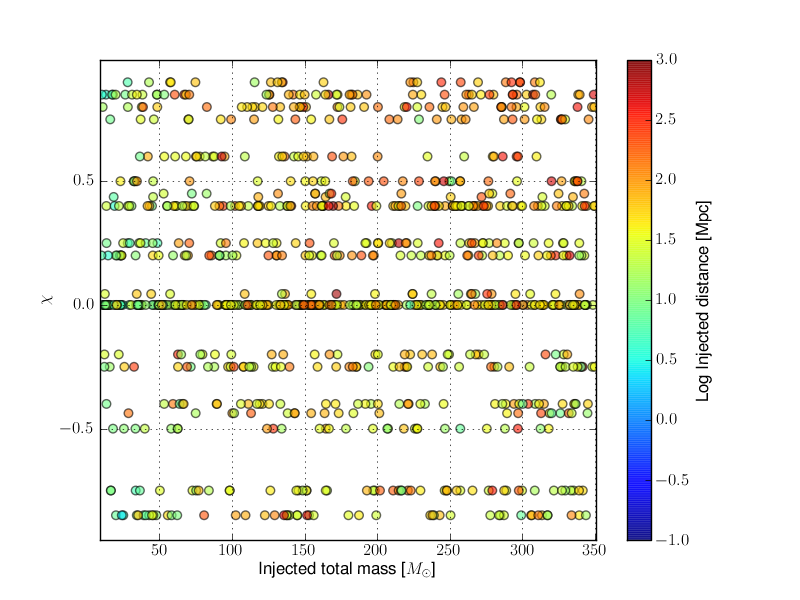
\includegraphics[width=\linewidth]{figures/ninja2/ninja2_dataset.png}
  \caption[Parameters of the NINJA-2 two-month data set]{
  \label{f:ninja2_dataset}
Distribution of mass, spin and distance parameters in the two-month,
Gaussian-noise data set.
}
\end{figure}%


As in NINJA-1 the sky location and inclination were chosen uniformly
at random.

For NINJA-2, in sharp contrast to NINJA-1, we created several two-week
test data sets in order to verify the waveforms and injection codes.
These tests were broken into smaller mass regions, ``low mass'' from
$10-40 \msun$, ``high-mass'' from $35-100 \msun$ and
``burst/ringdown'' from $80-350 \msun$.  The original intent had been
to create three full 2-month data sets along these same lines, but
that proved to be infeasible due to the file size of the data sets.
However, it was useful in the test sets as it allowed several
pipelines to do sanity checks in the mass region to which they are
most sensitive.  These tests exposed several bugs in the injection
codes which were fixed before generating the two-month data set.

Real detector data is far from Gaussian, and real data analysis is
concerned not only with foreground triggers from signals but also
background triggers from noise.  In order to comprehensively test the
ability of pipelines to detect signals and recover their parameters it
is necessary to perform injections into real detector noise.  As of
this writing a memorandum of understanding (MoU) between the NINJA
collaboration, the LIGO collaboration and the Virgo collaboration has
been signed which will allow subsequent NINJA-2 data sets to use data
from the previous (S5/VSR1) science run as noise.  A key feature of
this agreement is that NINJA is not a gravitational-wave search.  We
will therefore use data from disjoint periods in each instrument.
Details of this plan, such as which times to use, have yet to be
decided.  However it is clear we will need a custom segment database
(see chapter~\ref{ch:detchar}) to mark times where the instruments
were glitching. However, injection times will not use this
information, as it is entirely possible that real signals will land on
or near a glitch, and the ability to detect such signals is an
important test.
 
There are two motivations for constructing and distributing the data
sets as NINJA-1 and NINJA-2 thus far have done.  The first is to
ensure that every group is looking at the same set of injections so
that results can be compared.  The second is due to the terms of the
NINJA agreement, which restricted distribution of the raw NR
waveforms.  However, distribution of such static sets limits the
ability of individual groups to tune their pipelines in optimal ways,
and conceptually distributing a set of parameters would be sufficient
to compare results across pipelines.  In addition the size of the data
sets makes distribution slow and complex.  The NR groups within NINJA
have therefore relaxed the conditions on their use of their waveforms.
Consequently, subsequent NINJA-2 data sets will be distributed as sets
of parameters, and data analysis groups will use the available code to
either create data sets locally, or perform the injections ``on the
fly'' as the analysis is performed.  This will also allow groups to do
special-purpose tuning runs or analyses, the results of which may be
published as short-author papers subject to the conditions of the
NINJA agreement.


\section{Data analysis}

As of this writing 12 groups have signed up to run analyses on the
NINJA-2 data.  Nine of these are running detection pipelines, listed
in table~\ref{tab:ninja2_detection}, and three are parameter
estimation pipelines, listed in
table~\ref{tab:ninja2_parameter_estimation}.  The detection pipelines
include a number of variations of the current CBC search described in
chapter~\ref{search} using different template families.  There is also
a matched filter ringdown search, a next-generation matched filter
search (GSTLAL) currently under development, and several unmodeled
burst searches.  As of this writing no analyses have competed
entirely, although several have been run on the test data sets as
sanity checks on the waveforms and injection process.  A few analyses
on the full two-month set have been run and preliminary results
reported, but none of these results have been analyzed beyond making
initial plots.  We restrict attention to results obtained from the
standard CBC search and refer to the NINJA-2 paper to be published in
2012 for the results from the full analyses and comparisons.

%
\begin{table}
\begin{center}
\begin{tabular}{|l|l|}\hline
Group & Analysis \\\hline
Cardiff/Syracuse & Standard and extended CBC pipelines \\
GSTLAL & Matched filter, inspiral, merger and ringdown \\
 & spin-aligned templates \\
Urbino & Matched filter PhenSpinInspiralRD templates \\
UMass & Burst search with Omega pipeline \\
Washington State & CBC high-mass with coherent stage \\
Ringdown & Matched filter, ringdown templates \\
AEI Hannover/UF Waveburst & Burst search with coherent Waveburst \\
UMD & CBC high-mass with EOBNRv2 templates \\
AEI/RIT & Matched filter search using spinning \\
 & phenomenological templates. \\
\hline
\end{tabular}
\end{center}
\caption[The detection pipeline analyses for NINJA-2.]{
\label{tab:ninja2_detection}
The detection pipeline analyses for NINJA-2}
\end{table}%


%
\begin{table}
\begin{center}
\begin{tabular}{|l|l|}\hline
Group & Analysis \\\hline
Northwestern/MIT & Parameter estimation with LALInference \\
inspnest & Parameter estimation and model selection \\
 & with nested sampling \\
\hline
\end{tabular}
\end{center}
\caption[The parameter estimation analyses for NINJA-2.]{
\label{tab:ninja2_paramater_estimation}
The parameter estimation analyses for NINJA-2}
\end{table}%

\subsection{CBC preliminary results}

The NINJA-2 data was analyzed with the standard CBC low-mass and
high-mass pipelines.  The parameters were exactly as in the S6/VSR2,3
runs, no changes were made to the configurations except for those
relating to the names of the data files.  The low-mass search uses
Taylor F2 templates to 3.5 pN order in phase evolution
(section~\ref{pn}) in a mass region defined by minimum component
masses of $1 \msun$ and maximum total mass of $25 \msun$.  The high
mass search uses EOBNR templates (section~\ref{eob}) in a region
defined by minimum component masses of $1 \msun$, minimum total mass
of $25 \msun$, and maximum total mass of $100 \msun$.  Plots of found
and missed injections are shown in figure~\ref{f:ninja2_cbc_results}.
\Note{Need to explain the V1 low mass results!}

\begin{figure}
  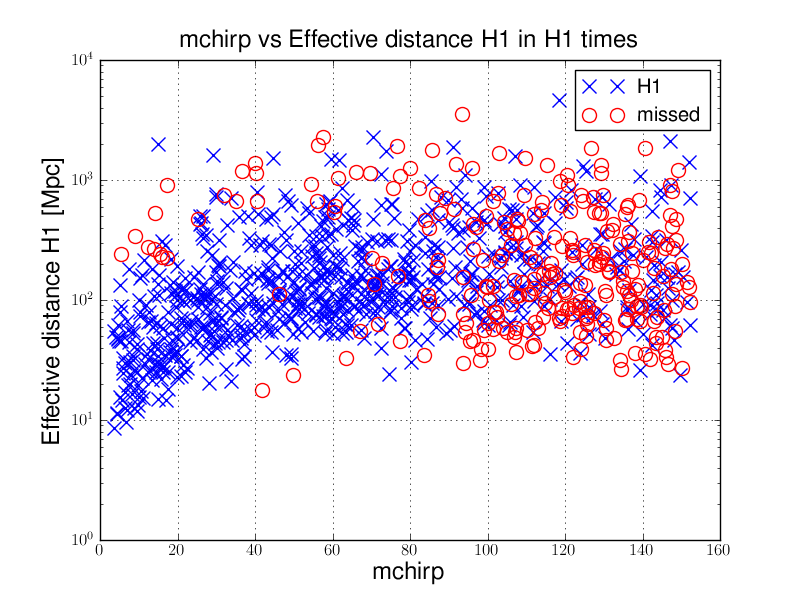
\includegraphics[width=0.5\linewidth]{figures/ninja2/H1-plotinspmissed_LOW_FULL_DATA_mchirp-eff_dist-log-H1-871147552-5209912.png}
  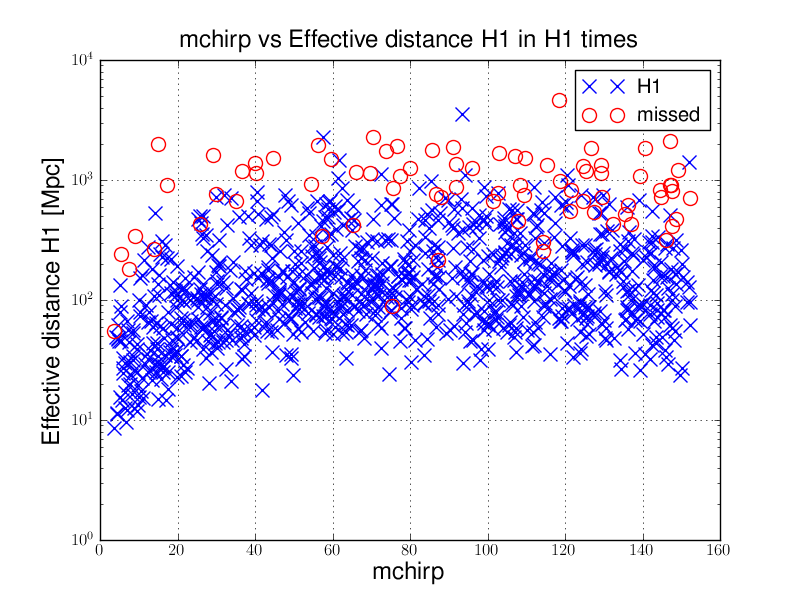
\includegraphics[width=0.5\linewidth]{figures/ninja2/H1-plotinspmissed_HIGH_FULL_DATA_mchirp-eff_dist-log-H1-871147552-5209912.png} \\
  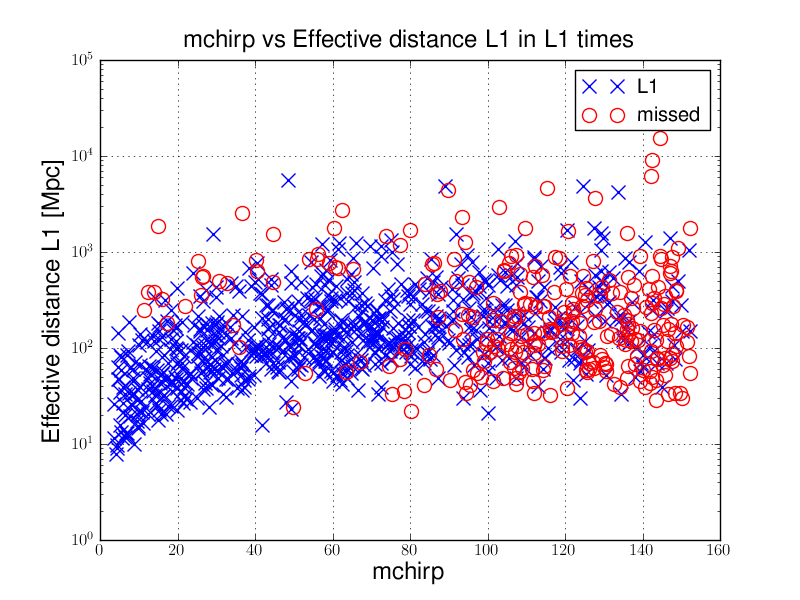
\includegraphics[width=0.5\linewidth]{figures/ninja2/L1-plotinspmissed_LOW_FULL_DATA_mchirp-eff_dist-log-L1-871147552-5209912.png}
  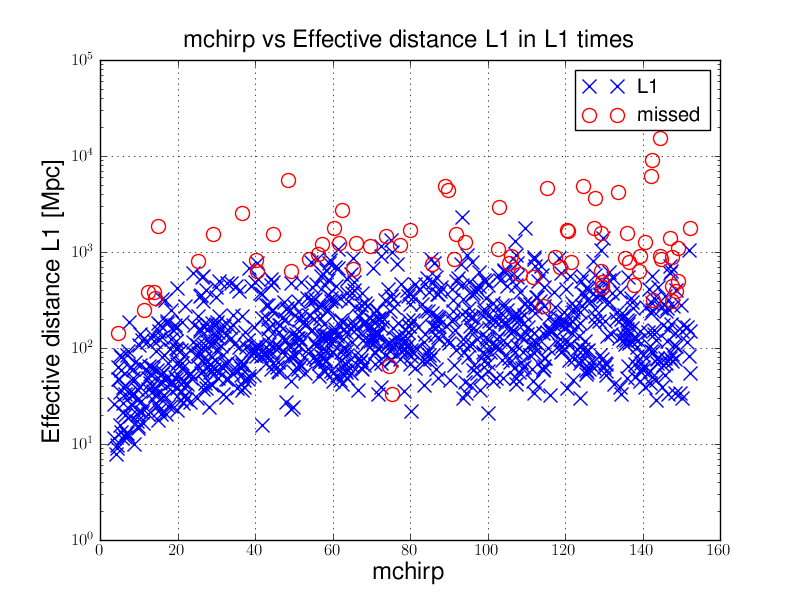
\includegraphics[width=0.5\linewidth]{figures/ninja2/L1-plotinspmissed_HIGH_FULL_DATA_mchirp-eff_dist-log-L1-871147552-5209912.png} \\
  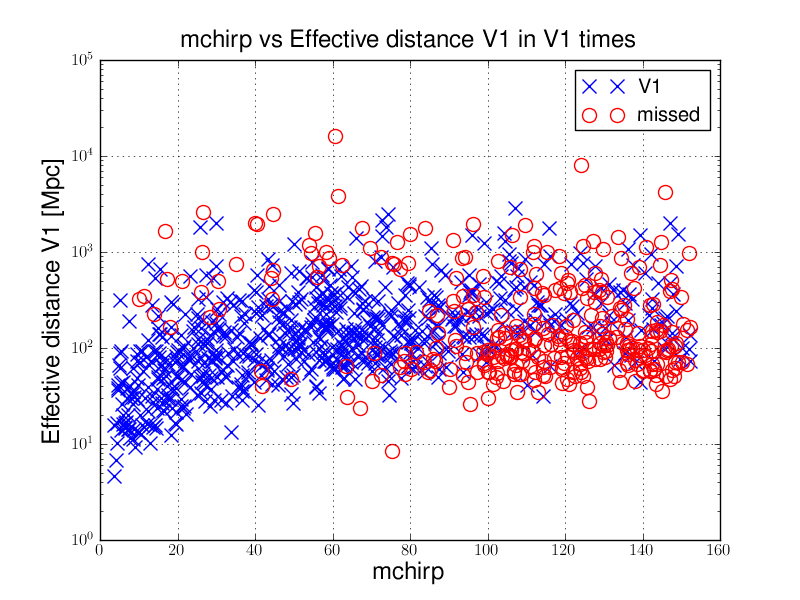
\includegraphics[width=0.5\linewidth]{figures/ninja2/V1-plotinspmissed_LOW_FULL_DATA_mchirp-eff_dist-log-V1-871147552-5209912.png}
  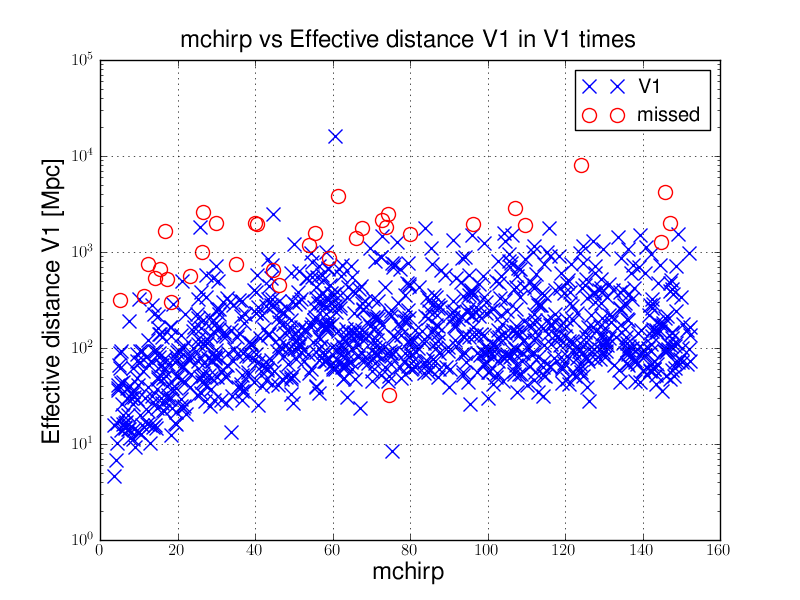
\includegraphics[width=0.5\linewidth]{figures/ninja2/V1-plotinspmissed_HIGH_FULL_DATA_mchirp-eff_dist-log-V1-871147552-5209912.png} \\
  \caption[Preliminary NINJA2 CBC results]{
  \label{f:ninja2_cbc_results}
Preliminary results from the CBC low-mass (left) and high-mass (right)
pipelines on the two-month NINJA-2 data set.
}
\end{figure}%


Show efficiency as a function of mass

Restrict to non-spinning signals and repeat



% TODO:
% make tables of submissions
% plot of paramater space in eta, chi scaled to 10 M
% plot of injection set (use chi instead of sum of magnitudes)
% text
% results
% explain move to 16384 (plot showing aliasing)
% explain longer data set (to get more statistics, allow
% self-blinding)

